\documentclass[/home/jesse/Analysis/FemtoAnalysis/AnalysisNotes/AnalysisNoteJBuxton.tex]{subfiles}
\begin{document}

\subsection{Fit Method Comparisons}
\label{App_ResultsLamK_FitMethComp}

The figures in this appendix show comparisons of extracted fit parameters obtained using different fit techniques.
Fig. \ref{figApp:Comparisons_3v10vNo} shows a comparison of results obtained using three, ten, and no residual contributors.
In Fig. \ref{figApp:Comparisons_FreevFixlam}, we demonstrate the effect of fixing the overall $\lambda_{\mathrm{Fit}}$ parameter compared to allowing it to be free (see Eq. \ref{eqn:CfwRes} in Sec. \ref{ResidualCorrelations}).
Fig. \ref{figApp:Comparisons_NormvStav} compares our normal fit results to those obtained when the correlation functions are built using the Stavinskiy method (see Sec. \ref{StavCfConstruction}).
Fig. \ref{figApp:Comparisons_SharevSepR} shows the difference between sharing radii among all \LamK systems versus only sharing radii between the \LamKpm systems.
Finally, Fig. \ref{figApp:Comparisons_ExpvSimXi} shows the effect of using the experimental $\Xi^{-}$\Kpm data compared to modeling it with a Coulomb-only curve for use in the residuals treatment (see Sec. \ref{ResidualCorrelations}).

All of the figures follow the same four-panel structure:
[Top Left]: $\Im f_{0}$ vs. $\Re f_{0}$, together with $d_{0}$ to the right.  [Top Right (Bottom Left, Bottom Right)]: $\lambda$ vs. Radius for the 0-10\% (10-30\%, 30-50\%) bin.
The \LamKchP system is always presented with red markers, the \LamKchM with blue, and the \LamKs with black.
In the case of all \LamK analyses sharing radii, the markers are gold.
In the case of only the \LamKpm analyses sharing radii, the markers are magenta.
The square symbols in the first column of the legends are to signify the color scheme.
The black symbols in the second column of the legend describe the fit procedure used.

To better explain the description in the legends, take Fig. \ref{figApp:Comparisons_3v10vNo} as an example. 
The square symbols in the first column of the top left figure indicate that the \LamKchP scattering parameters are shown in red, the \LamKchM in blue, and the \LamKs in black.
The symbols in the second column of the top left figure indicate that the case of three residual contributors is shown with closed circles, ten residual contributors with open crosses, and no residuals with open triangles.
For the $\lambda$ vs. radii plots, the square symbol describing the color scheme in the first column of the top right figure shows that all \LamK analyses share common radii and are shown with gold markers.

Fig. \ref{figApp:Comparisons_SharevSepR} is a bit more involved example, in terms of the markers, so it is worthwhile to explain as a second example.
The square symbols in the first column of the top left figure indicate that the \LamKchP scattering parameters are shown in red, the \LamKchM in blue, and the \LamKs in black.
The symbols in the second column of the top left figure indicate that the case where all \LamK analyses share common radii is shown with closed circles, the case of only \LamKpm analyses sharing radii is shown with open crosses, and the \LamKs system being fit alone is shown with open triangles.
For the $\lambda$ vs. radii plots, the square symbols describing the color scheme in the first column of the top right figure show that the case where all \LamK analyses share common radii is drawn with gold (in addition to being closed circles, as just described) markers, only \LamKpm analyses sharing radii is shown with magenta (in addition to open crosses, as just described) markers, and the \LamKs system being fit alone is shown with black (in addition to open triangles, as just described) markers.

%%%%%%%%%%%%%%%%%%%%%%%%%%%%%%%%%%%%%%%%%%%%%%%%%%%%%%%%%%%%%%%%%%%%%%%%%%%%%%%%%%%%%%%%%%%%%%%%%%%%%%%%%%%%%%%%%%%%%%%%%%%%
Fig. \ref{figApp:Comparisons_3v10vNo} shows a comparison of results obtained using three, ten, and no residual contributors.
A more detailed look of the fit with the experimental data can be found in Appendices \ref{App_ResultsLamK_3Res} - \ref{App_ResultsLamK_NoRes}.
As shown, the scattering parameters vary significantly between the different cases.
For the case of no residual contributors, we would expect the $\lambda_{\mathrm{Fit}}$ parameters to be closer to $\lambda_{\mathrm{Fit}} \sim$ 0.5, when considering the value extracted for primary pairs using simulation in Table \ref{tab:LambdaValues_All}.
For the case of 10 residual contributors, the figure shows the magnitude of the scattering parameters tends to increase, as do the $\lambda_{\mathrm{Fit}}$ parameters.
The improper treatment of the residuals places less emphasis on the primary interaction, as conveyed through the relative strength of the $\lambda_{\mathrm{Fit}}$ parameters between the three and ten residuals case, presented in Tab. \ref{tab:LambdaValues_All}.
More emphasis is placed on the residual contributors, whose signal is effectively flattened after being run through the appropriate transform matrices (as shown in Figs. \ref{fig:Sig0KchPtoLamKchPTransform} and \ref{fig:LamKSt0toLamKchPTransform} of Sec. \ref{ResidualCorrelations}).
This leads to a lot of mostly flat contributions, as shown e.g. in Fig. \ref{figApp:LamKchPwConjFitsAndResiduals_10Res} in App. \ref{App_ResultsLamK_10Res}.
These two effects could account for the (mostly) larger in magnitude scattering parameters and $\lambda_{\mathrm{Fit}}$ parameters extracted when assuming 10 residual contributors.


\begin{figure}[h]
  \centering
  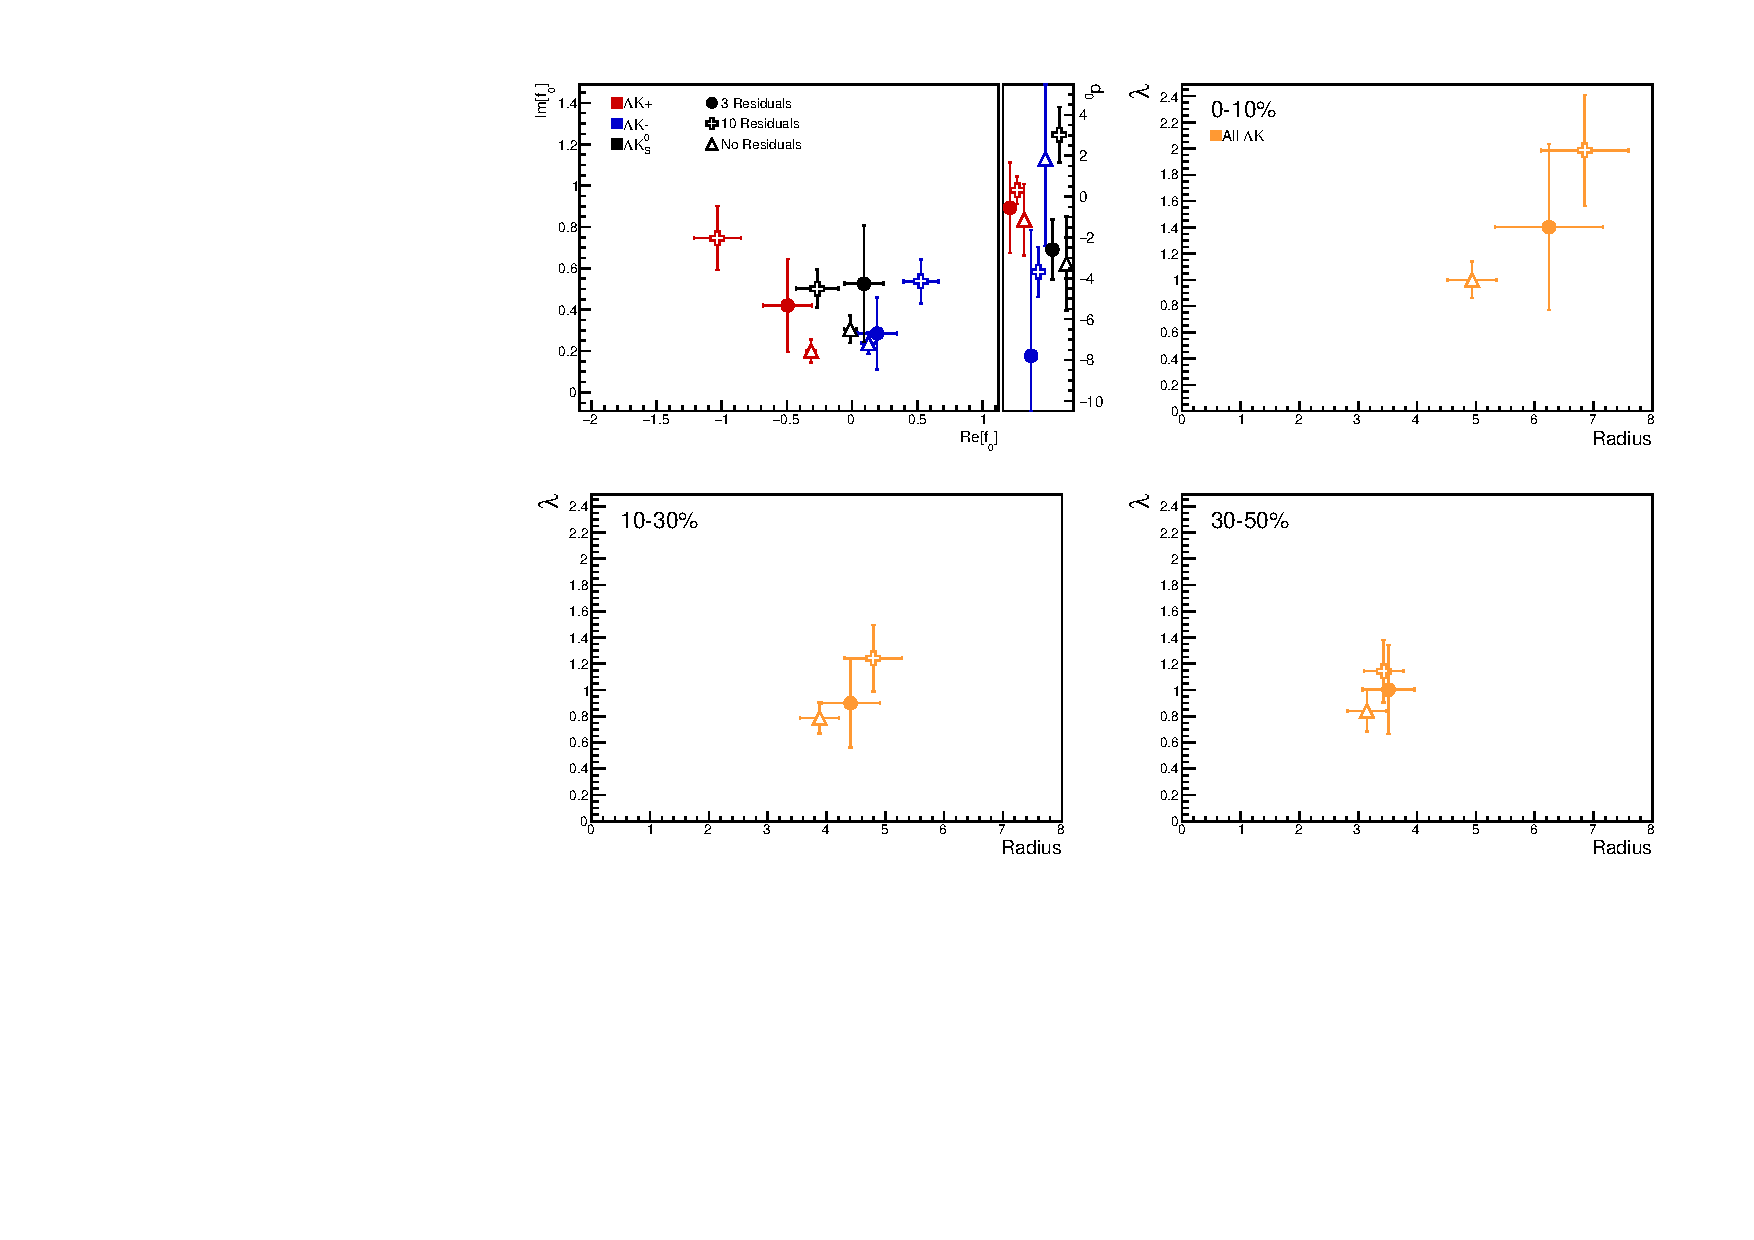
\includegraphics[width=0.75\textwidth]{/home/jesse/Analysis/Dissertation/Appendices/Appendix_Results/App_ResultsLamK_FitMethodComparisons/Figures/Comparisons_3v10vNo_StatOnly.pdf}
  \caption[Fit comparison: number of residuals]
  {
  Results shown for the case of 3 (closer, circles), 10 (open, crosses), and no (open, triangles) residual contributors included in the fit.
  See text at beginning of section for color scheme information.
  }
  \label{figApp:Comparisons_3v10vNo}
\end{figure}


%%%%%%%%%%%%%%%%%%%%%%%%%%%%%%%%%%%%%%%%%%%%%%%%%%%%%%%%%%%%%%%%%%%%%%%%%%%%%%%%%%%%%%%%%%%%%%%%%%%%%%%%%%%%%%%%%%%%%%%%%%%%
In Fig. \ref{figApp:Comparisons_FreevFixlam} we demonstrate the effect of fixing the overall $\lambda_{\mathrm{Fit}}$ parameter compared to allowing it to be free (see Eq. \ref{eqn:CfwRes} in Sec. \ref{ResidualCorrelations}).
As shown, the extracted scattering parameters are mostly unaffected by this choice.
The radii behave as expected, when considering the $\lambda_{\mathrm{Fit}}$ and $R$ parameters are strongly correlated.
For instance, forcing $\lambda_{\mathrm{Fit}}$ to decrease, as in the 0-10\% centrality bin shown in the top right of the figure, causes the fit radius to also decrease.

\begin{figure}[h]
  \centering
  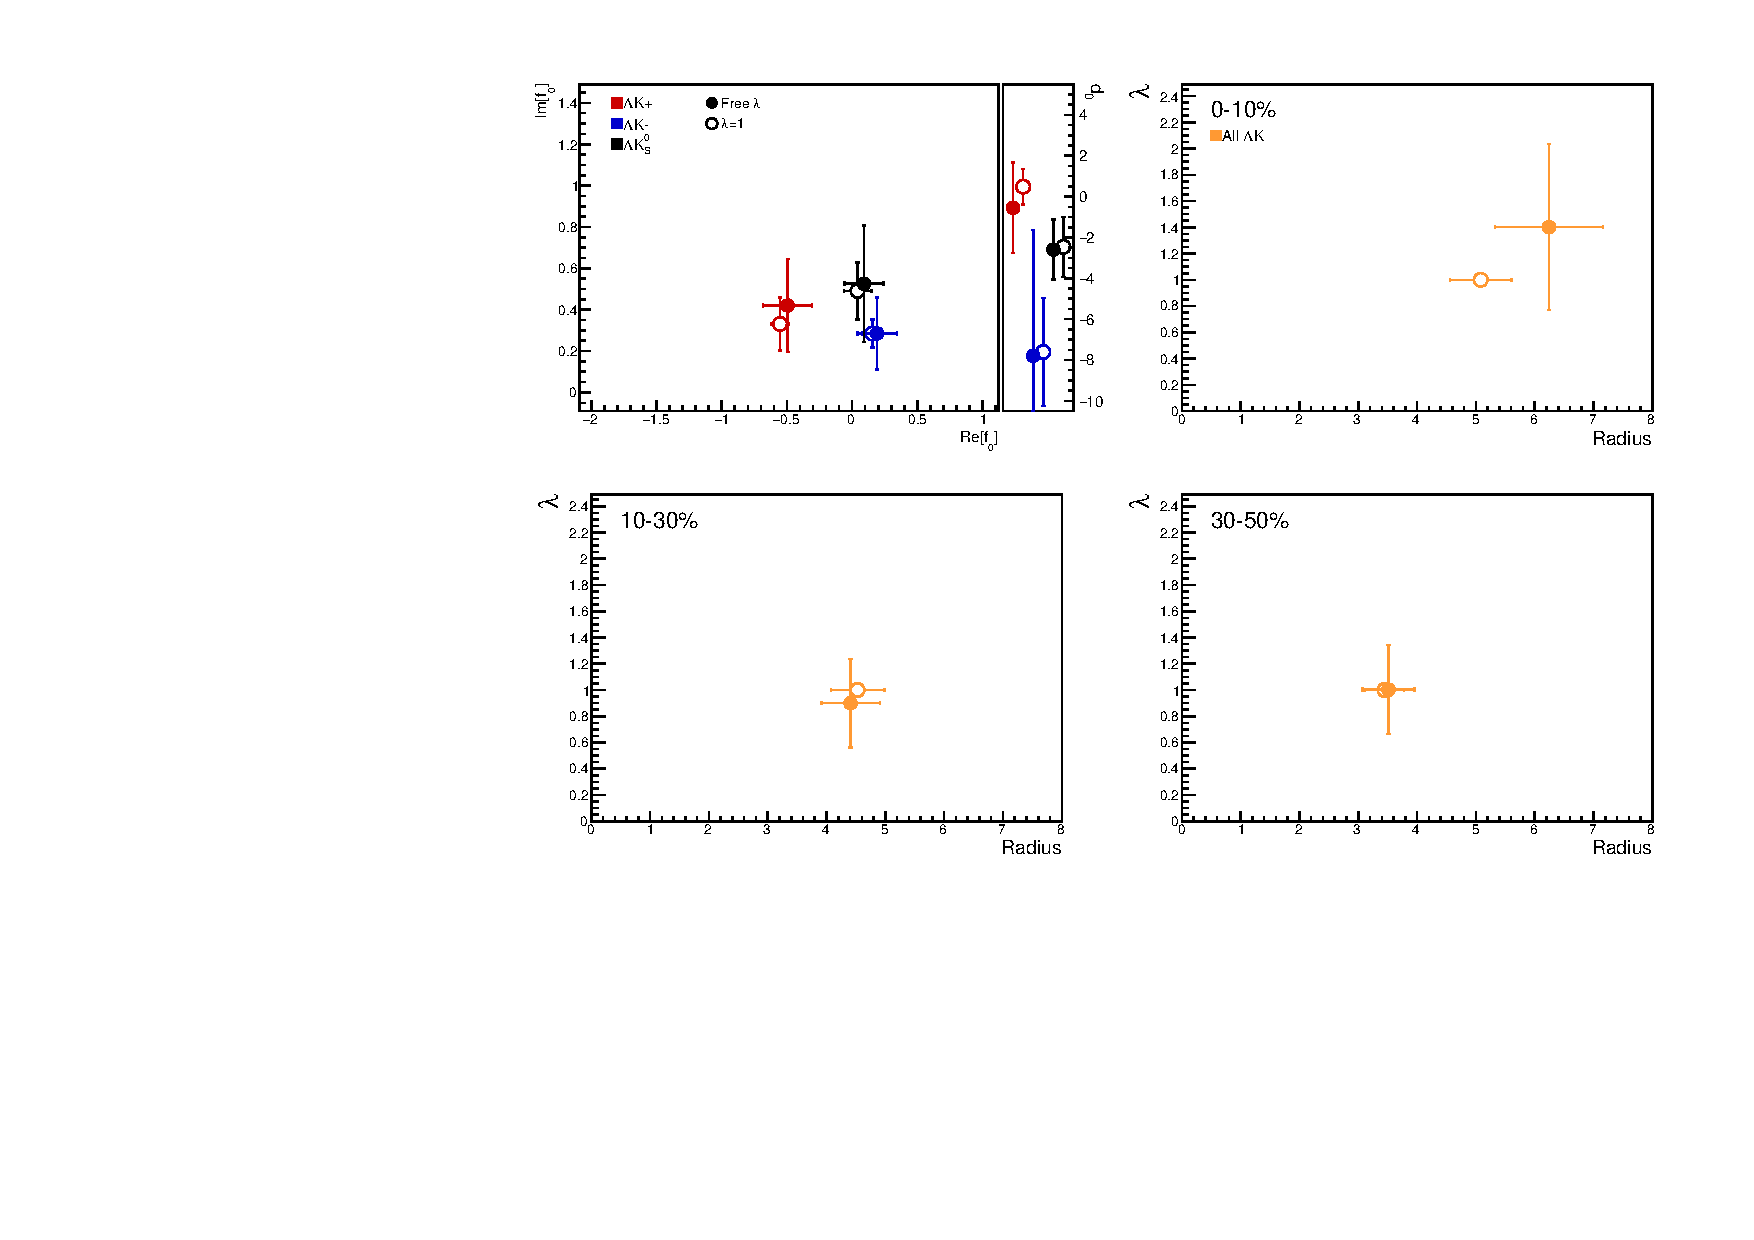
\includegraphics[width=0.75\textwidth]{/home/jesse/Analysis/Dissertation/Appendices/Appendix_Results/App_ResultsLamK_FitMethodComparisons/Figures/Comparisons_FreevFixlam_StatOnly.pdf}
  \caption[Fit comparison: free vs fixed $\lambda_{\mathrm{Fit}}$]
  {
  Results shown for $\lambda_{\mathrm{Fit}}$ parameters left free (closed, circles) and fixed to 1 (open, circles).
  See text at beginning of section for color scheme information and Eq. \ref{eqn:CfwRes} in Sec. \ref{ResidualCorrelations} for more information on the $\lambda_{\mathrm{Fit}}$ parameter.
  }
  \label{figApp:Comparisons_FreevFixlam}
\end{figure}



%%%%%%%%%%%%%%%%%%%%%%%%%%%%%%%%%%%%%%%%%%%%%%%%%%%%%%%%%%%%%%%%%%%%%%%%%%%%%%%%%%%%%%%%%%%%%%%%%%%%%%%%%%%%%%%%%%%%%%%%%%%%
Fig. \ref{figApp:Comparisons_NormvStav} compares our normal fit results to those obtained when the correlation functions are built using the Stavinskiy method (see Sec. \ref{StavCfConstruction}).
As shown in the figure, with the exception of the $d_{0}$ parameters (which are difficult for us to resolve experimentally), the results from the two methods are within errors of each other.
As implemented in this analysis, the Stavinskiy method does a good job of reducing the non-femtoscopic background, but does not completely eliminate it.
Nonetheless, it is a simple and elegant method, and should be investigated further in the future.

\begin{figure}[h]
  \centering
  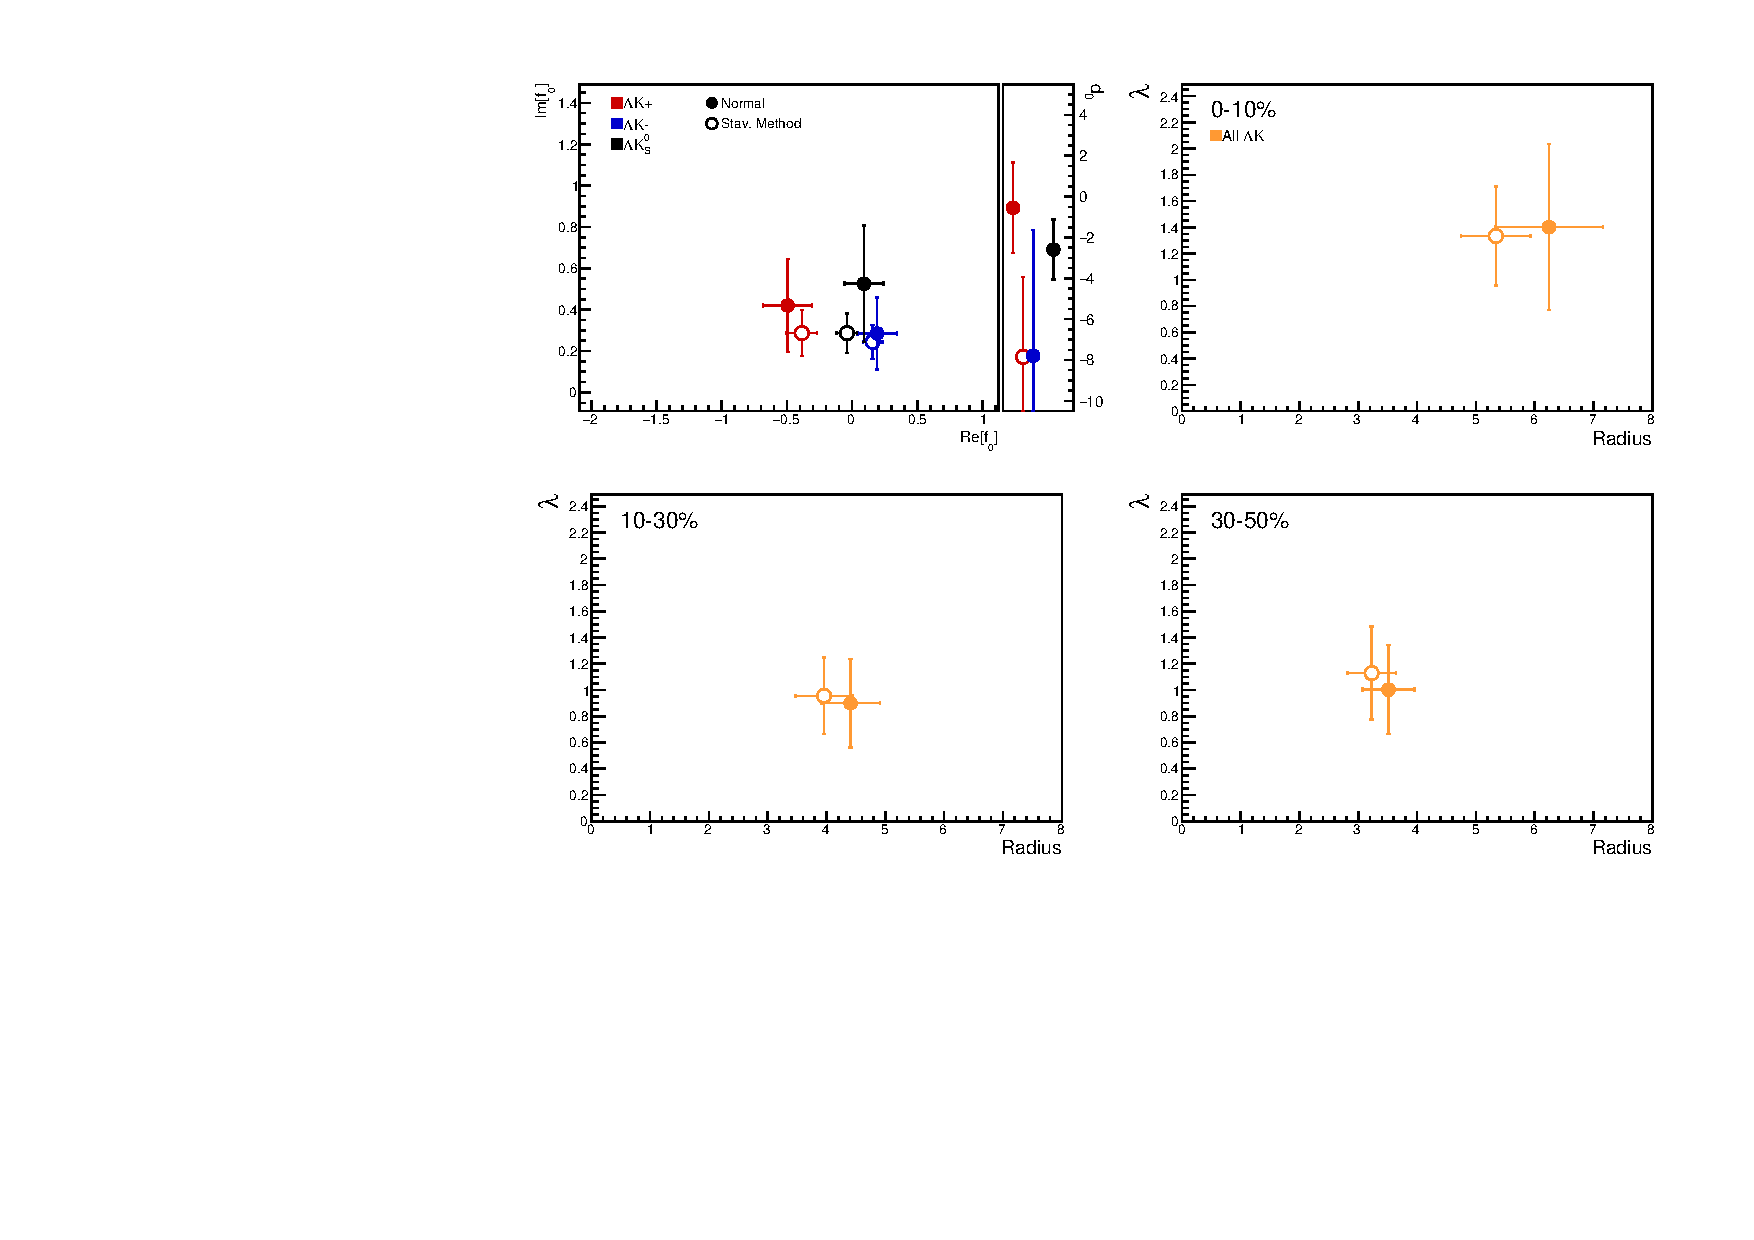
\includegraphics[width=0.75\textwidth]{/home/jesse/Analysis/Dissertation/Appendices/Appendix_Results/App_ResultsLamK_FitMethodComparisons/Figures/Comparisons_NormvStav_StatOnly.pdf}
  \caption[Fit comparison: normal CF construction vs. Staninskiy method]
  {
  Results shown for normal correlation function construction (closed, circles) and when built using the Stavinskiy method (open, circles).
  See text at beginning of section for color scheme information and Sec. \ref{StavCfConstruction} for more information on the Stavinskiy method.
  }
  \label{figApp:Comparisons_NormvStav}
\end{figure}


%%%%%%%%%%%%%%%%%%%%%%%%%%%%%%%%%%%%%%%%%%%%%%%%%%%%%%%%%%%%%%%%%%%%%%%%%%%%%%%%%%%%%%%%%%%%%%%%%%%%%%%%%%%%%%%%%%%%%%%%%%%%
Fig. \ref{figApp:Comparisons_SharevSepR} shows the different between sharing radii among all \LamK systems versus only sharing radii between the \LamKpm systems.
As shown in the figure, the \LamKpm systems give consistent results whether or not the \LamKs system is included in the fit.
The \LamKs system, however, gives significantly different results when fit by itself.
The \LamKs system suffers the most from low statistics, and is the most difficult to fit (for instance, when fit by itself, the $\lambda_{\mathrm{Fit}}$ parameter has to be limited between [0.6, 1.1] to give realistic results).
As shown, when fit alone, the \LamKs fit settles on much smaller radii compared to the \LamKpm systems.
As we expect the \LamKs system to share similar radii with the \LamKpm systems, we chose to join the three together to combat the low statistics available to the \LamKs.
The purpose of this figure is mainly to demonstrate how the inclusion of the \LamKs affects the \LamKpm results, not the other way around.

\begin{figure}[h]
  \centering
  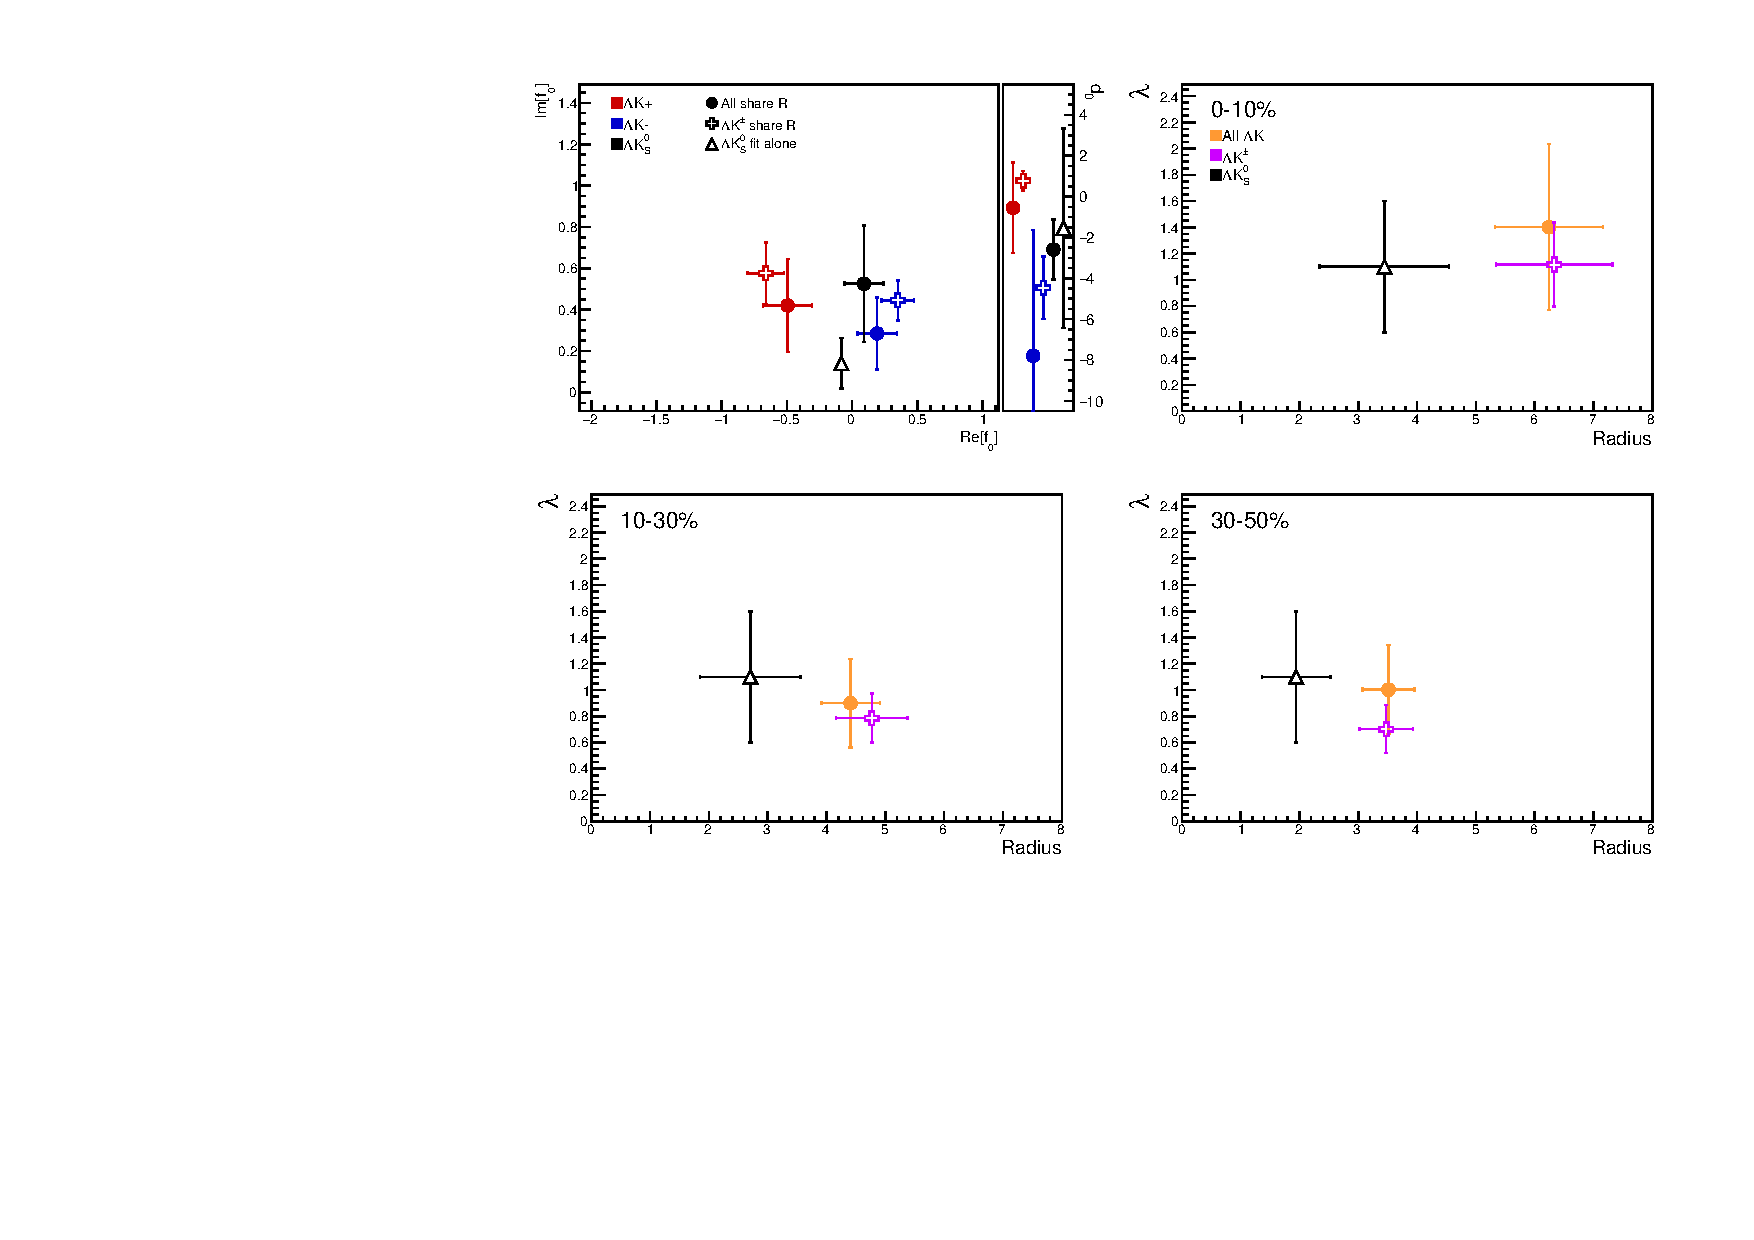
\includegraphics[width=0.75\textwidth]{/home/jesse/Analysis/Dissertation/Appendices/Appendix_Results/App_ResultsLamK_FitMethodComparisons/Figures/Comparisons_SharevSepR_StatOnly.pdf}
  \caption[Fit comparison: shared vs. separate radii]
  {
  Results shown for the case of all \LamK analyses sharing radii (closed, circles) and only the \LamKpm analyses sharing radii (open, crossed), with the \LamKs system fit separately (open, triangles).
  See text at beginning of section for color scheme information.
  }
  \label{figApp:Comparisons_SharevSepR}
\end{figure}


%%%%%%%%%%%%%%%%%%%%%%%%%%%%%%%%%%%%%%%%%%%%%%%%%%%%%%%%%%%%%%%%%%%%%%%%%%%%%%%%%%%%%%%%%%%%%%%%%%%%%%%%%%%%%%%%%%%%%%%%%%%%
Finally, Fig. \ref{figApp:Comparisons_ExpvSimXi} shows the effect of using the experimental $\Xi^{-}$\Kpm data compared to modeling it with a Coulomb-only curve for use in the residuals treatment (see Sec. \ref{ResidualCorrelations}).
As shown, the results are consistent.
The use of a the experimental data is preferable in that no assumption need to be made about the parent system's correlation function.
However, the low statistics of the parent $\Xi^{-}$\Kpm data (especially in the 30-50\% centrality bin) could be reason to instead use the Coulomb-only curve.
In our description, we choose to use the experimental data, although, as shown in the figure, the choice does not matter much.

\begin{figure}[h]
  \centering
  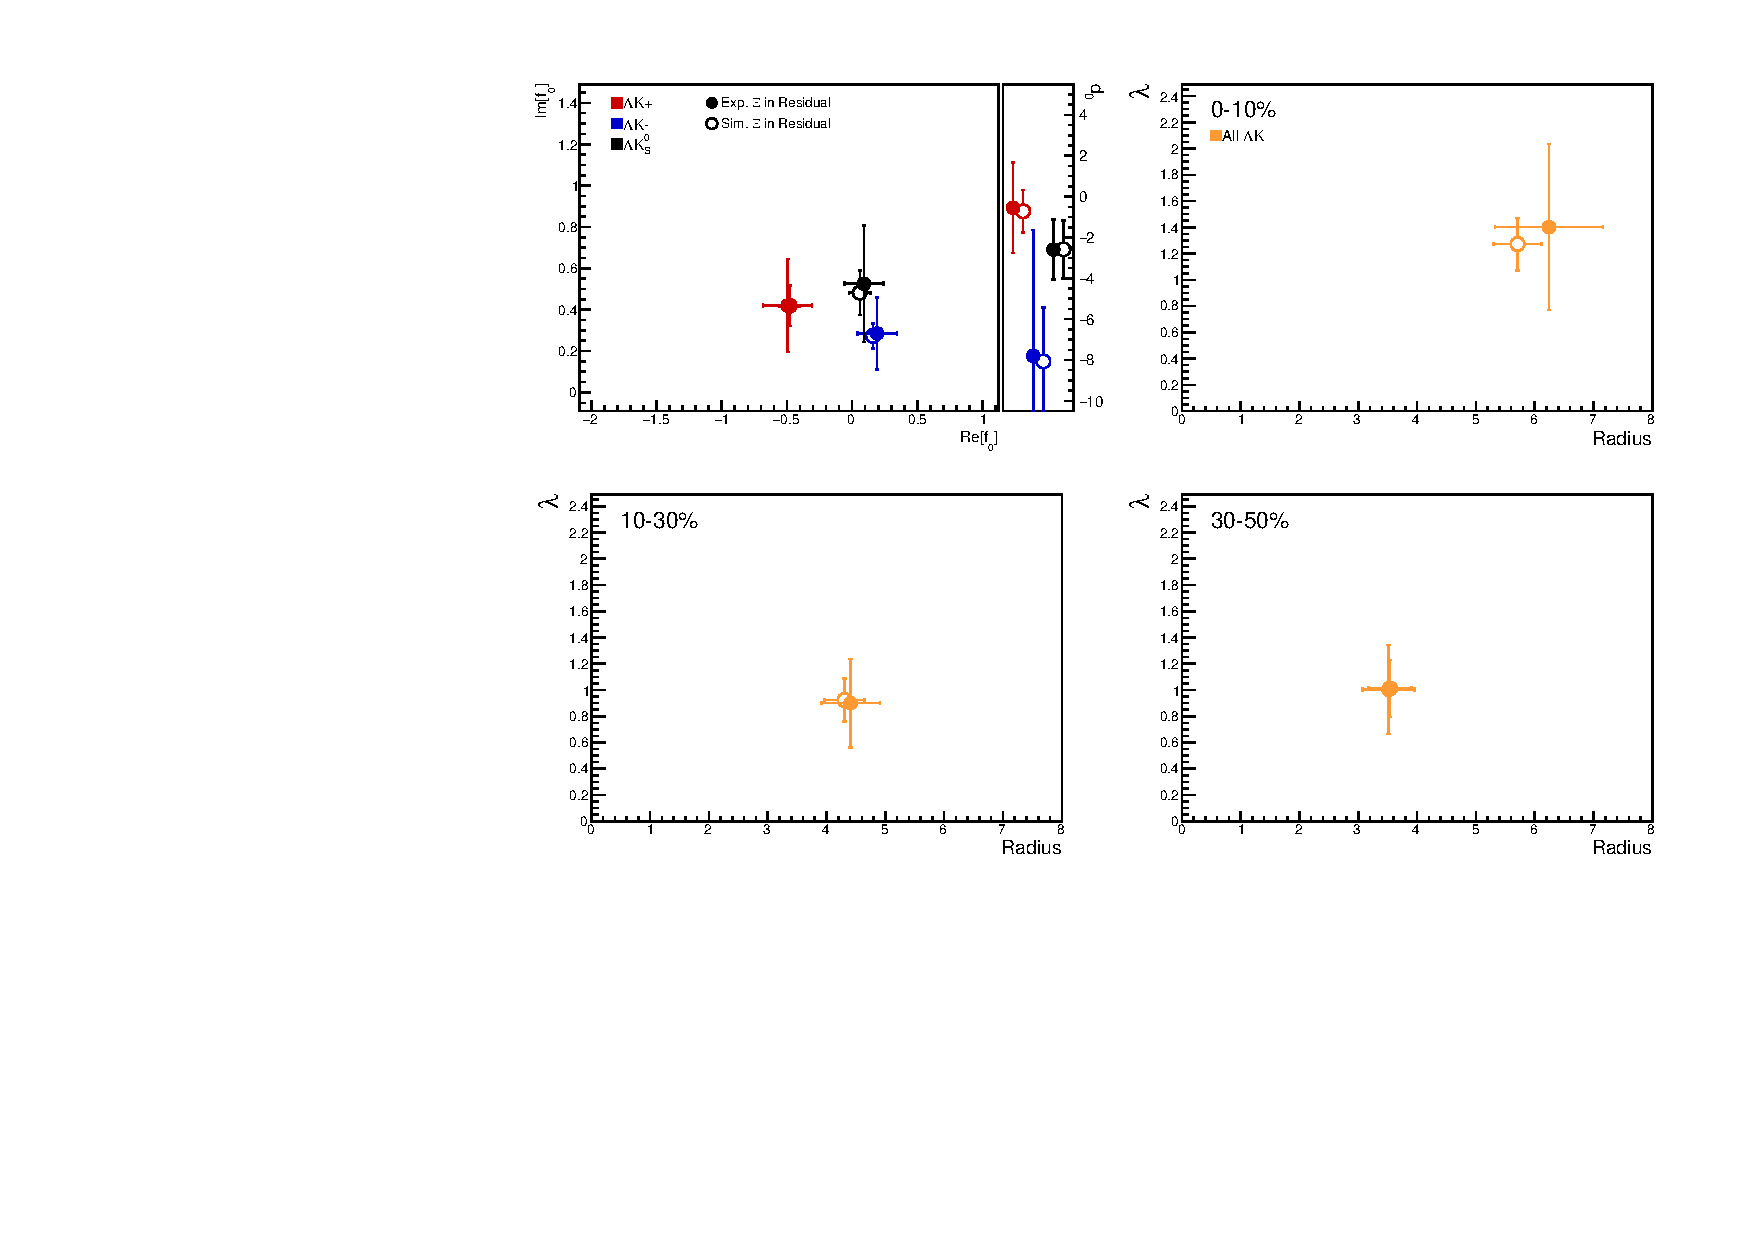
\includegraphics[width=0.75\textwidth]{/home/jesse/Analysis/Dissertation/Appendices/Appendix_Results/App_ResultsLamK_FitMethodComparisons/Figures/Comparisons_ExpvSimXi_StatOnly.pdf}
  \caption[Fit comparison: experimental vs simulated $\Xi^{-}$\Kpm]
  {
  Results shown when using experimental $\Xi^{-}$\Kpm data (closed, circles) and when simulating the $\Xi^{-}$\Kpm correlation function with a Coulomb-only curve (open, circles) for use in the treatment of the residual.  
  See text at beginning of section for color scheme information, and Sec. \ref{ResidualCorrelations} for more information on the $\Xi^{-}$\Kpm simulation.
  }
  \label{figApp:Comparisons_ExpvSimXi}
\end{figure}






%\clearpage
\end{document}